\section{Our Research} 

\subsection{Our Motivation}
\cite{o1998six}
O'Reilly presents what he thinks as biologically plausible. In the end of this review we provide citations from this article which shortly explain the most important concepts of NN design. 

Article also contains interesting references to several experiments. It also presents the Leabra model (PhD thesis of O'Reilly) which is presented as a base model for other NN which can be derived from Leabra. The question how to merge the proposed principles is dicussed, especially the case of competiveness and distributed representation. 

Biological realism. "Moreover, computational mechanisms that violate
known biological properties should not be relied upon. "

Distributed representations. "A distributed representation
uses multiple active neuron-like processing units to encode
information (as opposed to a single unit, localist represen-
tation), and the same unit can participate in multiple repre-
sentations. Each unit in a distributed representation can be
thought of as representing a single feature, with information
being encoded by particular combinations of such features.
"

Inhibitory competition. " Inhibitory competition arises when mutual
inhibition among a set of units (i.e. as mediated by in-
hibitory interneurons) prevents all but a subset of them
from becoming active at a time.  Furthermore, most learn-
ing mechanisms (including those discussed later) are
affected by this selection process such that only the selected
representations are refined over time through learning, re-
sulting in an effective differentiation and distribution of
representations. More generally, it seems as though the world can be usefully
represented in terms of a large number of categories with a
large number of exemplars per category (animals, furniture,
trees, etc.). "

Bidirectional activation propagation (interactivity). "They showed that
interactivity could explain the counterintuitive finding that
higher-level word processing can influence lower-level letter
perception. More recently, Vecera and O’Reilly showed
that bidirectional constraint satisfaction can model people’s
ability to resolve ambiguous visual inputs in favor of familiar
versus novel objects. "

Error-driven task learning. "Error-driven learning (also called ‘supervised’ learning) is
important for shaping representations according to task de-
mands by learning to minimize the difference (i.e. the error)
between a desired outcome and what the network actually
produced. "

Hebbian model learning. "that something like correlational structure is important.
Hebbian learning mechanisms represent this correlational
structure, encoding the extent to which different things co-
occur in the environment."

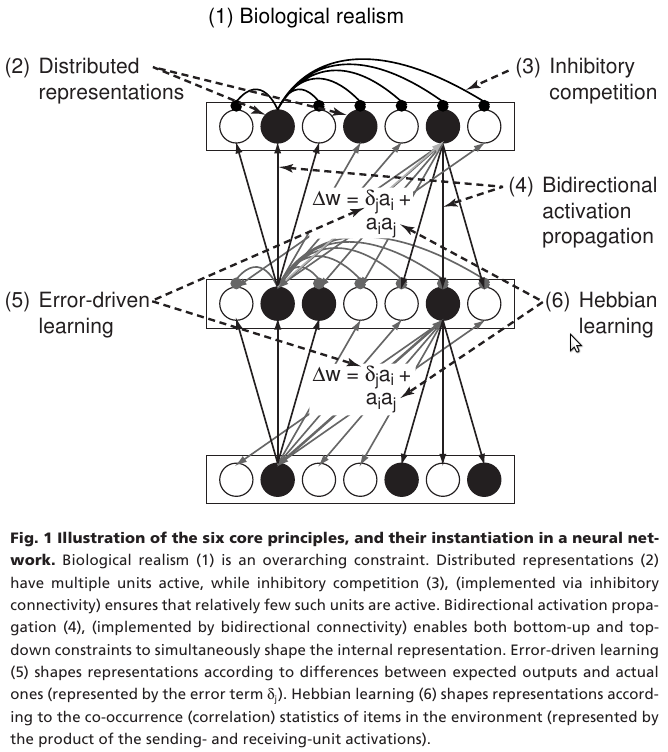
\includegraphics[width=12cm]{img/bio_plausability_o1998six.png}
